\chapter{引言}\label{cha:introduction}
%引言是论文正文的开端,应包括毕业论文选题的背景、目的和意义;对国内外研究现状和相关领域中已有的研究成果的简要评述;介绍本项研究工作研究设想、研究方法或实验设计、理论依据或实验基础;涉及范围和预期结果等。要求言简意赅,注意不要与摘要雷同或成为摘要的注解。
\section{选题背景与意义}
\label{sec:background}
医学影像中的疾病标记物是一种生物特征,或可在图像中检测到的疾病标志物。医学影像中的视觉疾病标记物是专业医师评估特定疾病的风险,类别和状态的重要指标。专业医师在诊断过程中,必然会遇到难以诊断的病例。而疾病标记物作为一种可以做出可靠诊断的有效手段,其实用性已经在临床使用中被证明。

在医学影像中,疾病标志物是与患者诊断相关的图像特征。例如,许多疾病标记物经常用于确定肺癌的风险。通过X射线,电子计算机断层扫描仪(Computed Tomography,缩写为CT)或核磁共振成像(Magnetic Resonance Imaging,缩写为MRI)检测到的简单的肺部病变可诊断为疑似肿瘤。病变本身可作为疾病标记物,病变的微小细节也可作为疾病标记物,并可共同用于评估肿瘤的风险。如肺结节评估中使用的一些成像疾病标记物包括大小、针刺、钙化、空化、肺内位置、生长速率和代谢速率,这些疾病标记物可综合诊断肺癌,以给出合理科学的诊断结果。除此之外,还可以使用多种技术(例如肺部CT或者MRI、脑电图、脑磁图、皮肤镜图像及其各种医学影像设备)测量成像疾病标记物。为了让读者对医学图像中的疾病标记物有较为直观的认识,如图\ref{mul_fig:medical_imaging_biomarkers_examplar}所示,本文列出了四张包含疾病标记物的眼底图像,由于眼底图像中疾病标记物分布较为广泛(比如,图中第一列图像),我们只标出图像中具有典型特性的疾病标记物。
%\begin{figure}[h!]
%	\centering
%	\begin{subfigure}{0.5\textwidth}
%		\centering
%		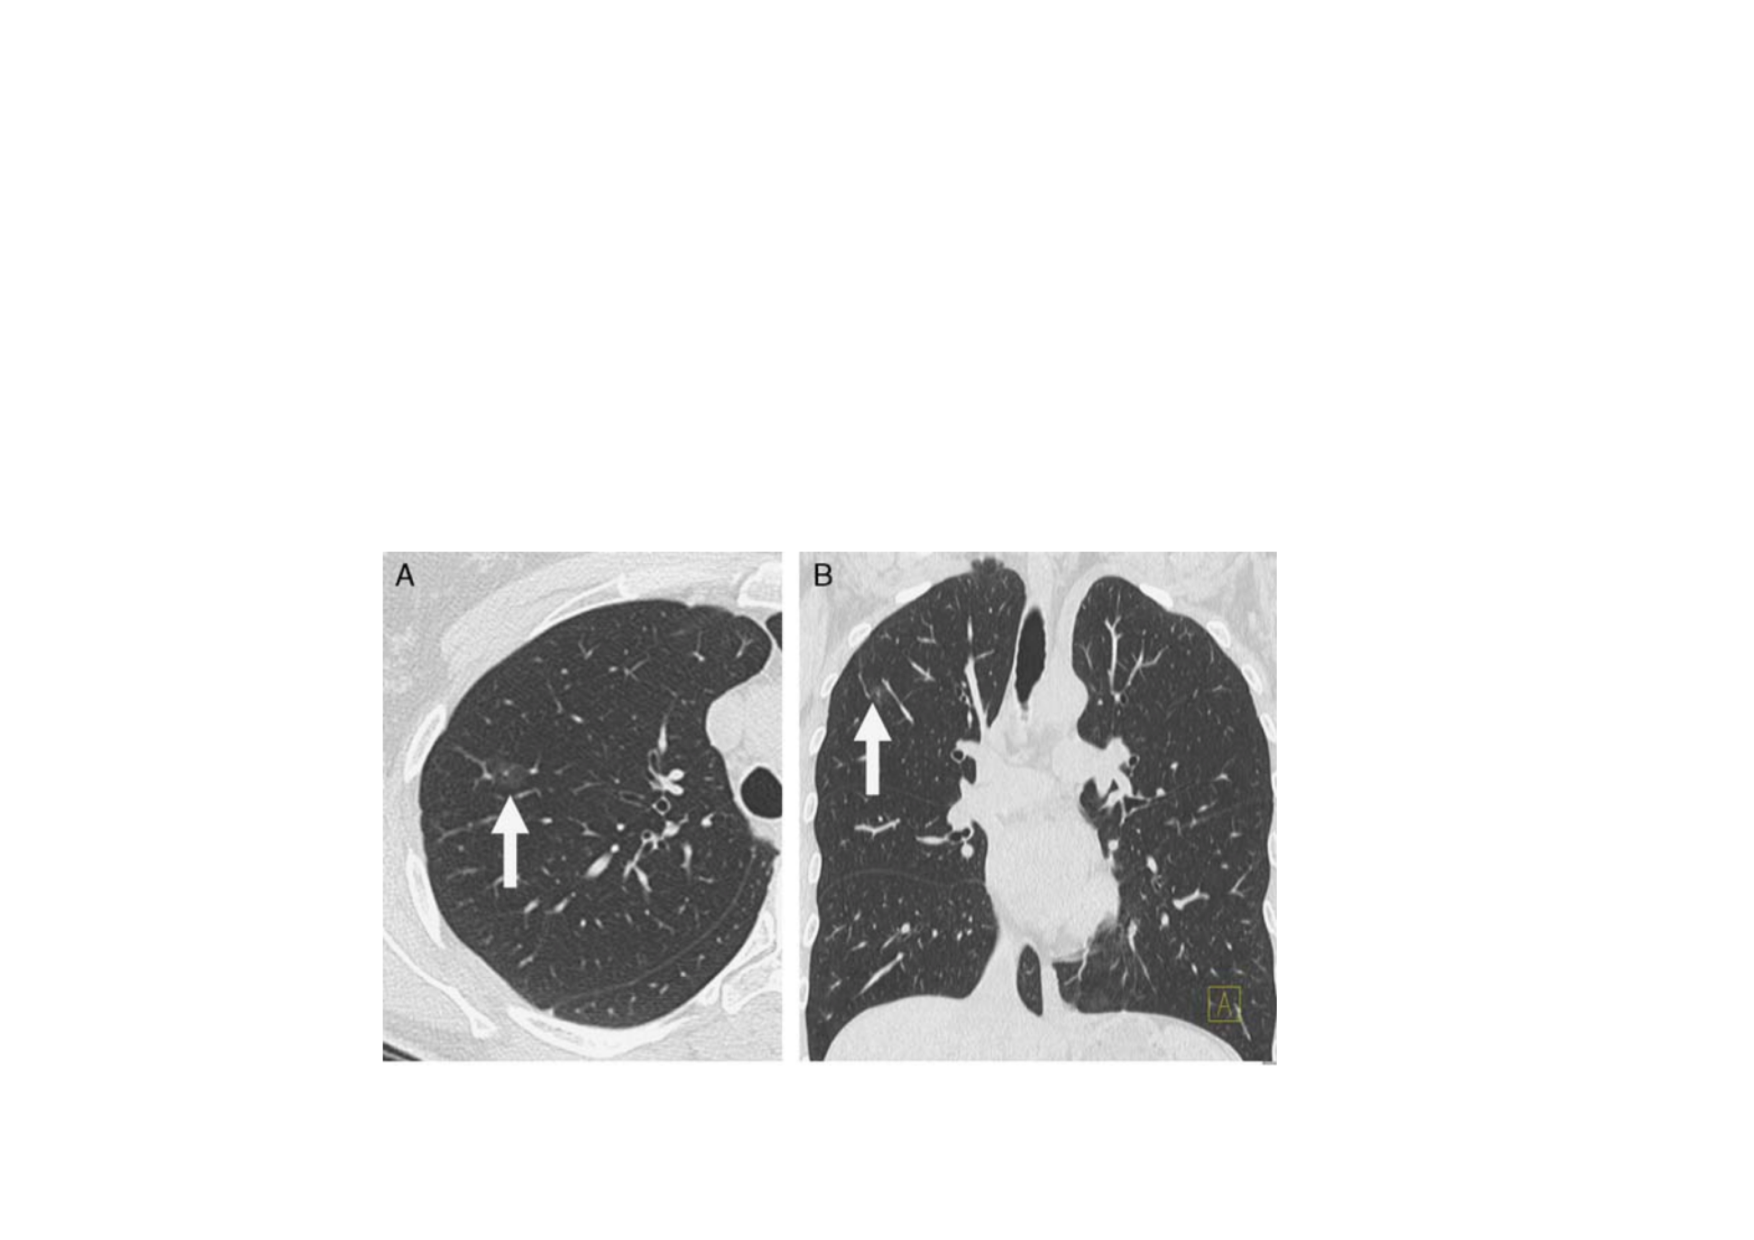
\includegraphics[width=1\textwidth]{figure/ground_glass_nodule}
%		\caption{玻璃结节。}
%		\label{subfig:ground_glass_nodule}
%	\end{subfigure}
%	\quad
%	\begin{subfigure}{0.462\textwidth}
%		\centering
%		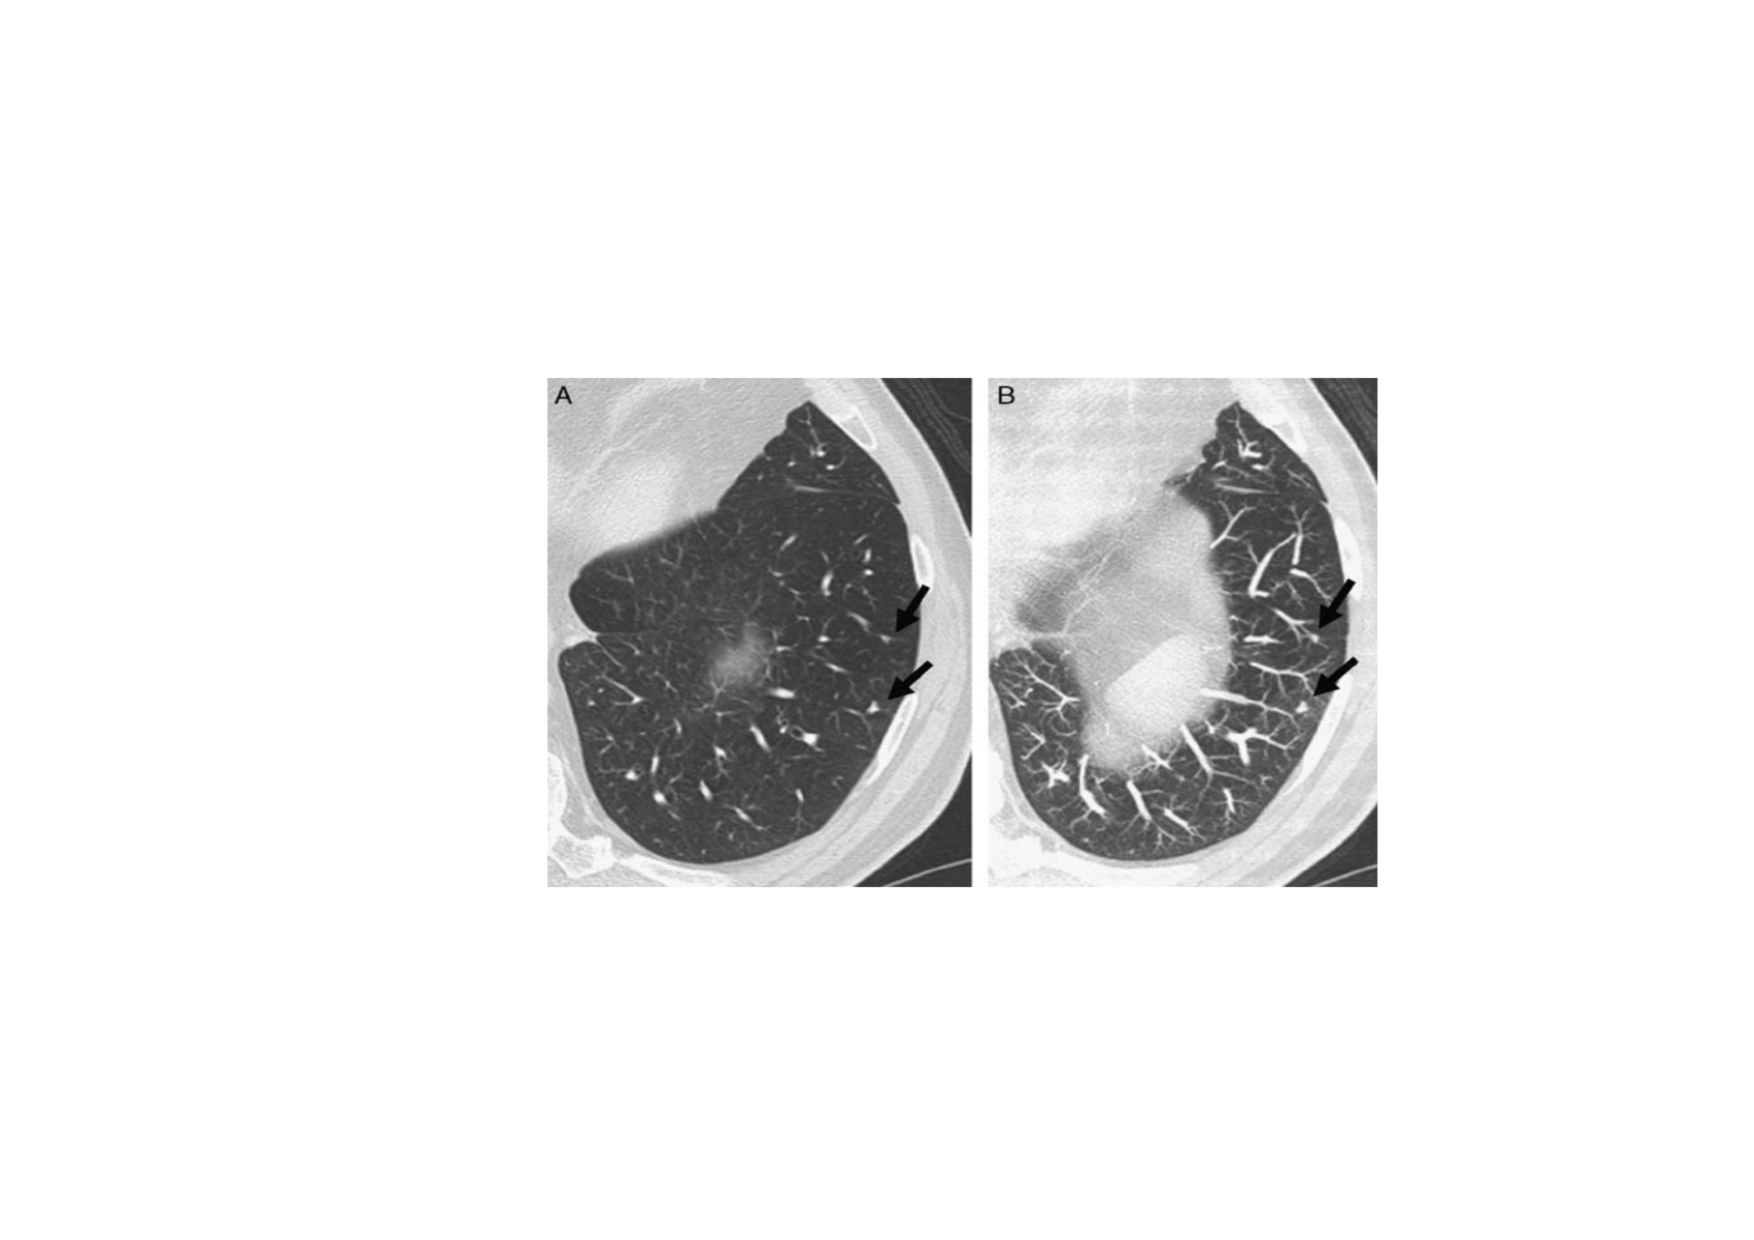
\includegraphics[width=1\textwidth]{figure/solid_nodule}
%		\caption{实性结节。}
%		\label{subfig:solid_nodule}
%	\end{subfigure}
%	\caption{医学影像中的疾病标记物示例(图片均来自于原文~\cite{brandman2011pulmonary})。以上图像均是肺部CT影像,均含有肺部结节,左侧子图中包含玻璃结节(白色箭头),右侧子图中包含玻璃结节(黑色箭头)。}
%	\label{mul_fig:medical_imaging_biomarkers_examplar}
%\end{figure}
\begin{figure}[h]
	\centering
	\includegraphics[width=1.0\textwidth]{figure/typical_biomarkers_examplar}
	\caption[眼底图像中的疾病标记物示例]{眼底图像中的疾病标记物示例(图中红色箭头指示疾病标记物)。}
	\label{mul_fig:medical_imaging_biomarkers_examplar}
\end{figure}

% 小分子疾病标记物:人体内的小分子物质非常多,食物中所含的氨基酸、葡萄糖、无机盐、维生素等均是小分子。这些小分子物质对于为止人体基本生命活动起着至关重要的作用,这些小分子化合物含量过高或者过低表明人体患有某项特定疾病。比如,血液中血糖长期处于较高水平表明极有可能患有糖尿病,低密度脂蛋白(俗称坏胆固醇)含量过高很可能会诱发冠心病。因此,这些小分子化合物在人体中发生的变化(含量变得过高或者高低)可以作为疾病诊断的有效依据。

% 大分子疾病标记物:人体内的大分子物质包括核酸、蛋白质和脂肪等。核酸主要指的是核糖核酸(缩写为RNA)的水平,是部分病毒、类病毒的遗传信息的载体和存在形式。当病毒入侵人体时,人体免疫系统会对病毒做出反应,分泌相关物质杀灭病毒,因而会引起病毒相关RNA水平的变化,因此RNA水平可反映出人体对入侵人体的病毒的反应状态。2020年春节期间我国武汉市集中爆发的肺炎病例确诊也是将冠状病毒的核酸序列对比检验作为诊断依据~\cite{corman2020detection}。蛋白质作为人体生命活动的主要参与者,参与到了生命活动的各个过程中,因此蛋白质也可看做是疾病标记物。同理,脂肪作为最重要的能量储备物质、身体的保护层,并且调节人体内分泌平衡,同样可看做是疾病标记物。

% 复合疾病标记物:复合疾病标记物包括脱氧核糖核酸(缩写为DNA)、DNA-蛋白质、蛋白质之间的复合体等。DNA是生物细胞内遗传信息的存在形式,是生物体不可缺少的一类生物大分子。DNA中不同的碱基排列序列代表了不同的遗传信息,而生物体内碱基由一种变为另外一种的现象称为基因变异(也叫做基因突变)。基因突变是生物体普遍存在的现象。现代医学已经证明,某一类的基因突变和某一类疾病之间存在密切联系。例如,临床统计表明,携带某种变异基因的人患有阿尔兹海默症的几率要高于不携带该种变异基因的人。疾病和基因的之间的关系还能解释有些吸烟的人患病风险却要低于不吸烟的人这一现象。因此,像DNA这种大分子化合物也可看做疾病标记物,用于疾病风险预测。

% 生物种群标记物:生物种群在人体中也大量存在,并在人的生命活动中发挥重要作用。比如,人体肠道中的双歧杆菌能合成多种人体生长发育所必须的维生素,还能利用蛋白质残渣合成氨基酸。我国最新研究也解释了肠道细菌和肥胖之间的关系,认为肥胖可能由细菌引起~\cite{zhou2019xiao}。因此,人体内的生物种群可也反应人体状况,可作为疾病标记物。

疾病标记物在临床医学中可发挥重要作用,可用于处理疾病诊断、疾病风险预测、疾病类型区分等多个问题。而利用计算机技术在医学影像上实现对疾病标记物的自动定位,可为发现更多潜在疾病标记物提供技术支持,同时也能为影像科医师减轻一定工作量,有利于将影像科医师从繁重的工作中解放出来。
%医学中应用临床疾病治疗和诊断更加方便、更加快捷,更多造福人类社会。
%\section{研究现状}
%\label{sec:related_work}
%近年来,由于疾病标记物对于临床医学的重要作用,疾病标记物定位任务,最开始是在医学领域提出,常用的方法有蛋白质组学技术~\cite{srinivas2002proteomics}、鸟枪蛋白质组分析~\cite{hu2008salivary} 、靶向代谢组学解析~\cite{griffiths2010targeted}等生化方法。随着CT、MRI、X射线等成像设备的临床应用,不同疾病的影像数据不断涌现。由于医学影像标注的高昂成本,大量未标注的医学影像数据亟待有效处理与分析。近些年计算机算力的极大提升,加上海量医学影像数据,利用计算机技术从海量影像数据中找到疾病对应的疾病标记物的方法呼之欲出。实际上,很多机器学习方法~\cite{huynh2012statistical, he2010stable, mamoshina2018machine, swan2013application}和深度学习方法~\cite{yao2016imaging, zafeiris2018artificial, li2019efficient}已经被提出用于发现疾病标记物,在此不再多做赘述。而对于在弱监督条件下的疾病标记物定位问题,常见的有多示例学习(Multiple Instance Learning,缩写为MIL)和CNN的可视化这两种解决思路,除此之外,计算机视觉领域也提出了一系列弱监督目标定位方法。下面分别予以阐述。

% overview of weakly supervised object localization:https://www.jianshu.com/p/e0097769f3b3

%\subsection{多示例学习}
%MIL~\cite{maron1998framework}是一种常见的用于处理弱监督问题的方法。MIL方法通过训练一个二分类器,不仅完成对异常影像的判断任务(异常/正常),而且可粗略定位异常影像中的显著性区域(即待选疾病标记物)。因此,MIL方法可解决医学影像领域中的诸多问题,比如,眼底图像中的视网膜神经纤维分割~\cite{manivannan2017subcategory}和数字病理图像中的癌症诊断~\cite{kandemir2014empowering}。给定一张医学影像,根据MIL思想,将单张影像看作示例包,而对单张影像进行分块操作得到小方块,再将这些小方块看作一个个示例。从而将问题转化为在示例包标签已知情况下,找出示例(待选区域)的标签,最终将其中置信度最高的异常示例看作是疾病标记物。但是这种方法存在诸多缺点,首先对单张图像进行分块不易操作,分块尺寸过大时,精确度不够,很可能会包括较多正常区域,出现假阳现象;当分块尺寸过小时,很可能会漏掉异常区域,造成漏检现象,还会产生较多示例,大大增大后续训练的计算量和计算复杂度,因此,MIL方法也只能用于粗略定位图像中的目标物(例如,疾病标记物)。另外,当处理多类问题时,示例包就会出现多标签,使得问题变得大大复杂。因此,近些年来,这种思路少有人问津。

%\subsection{卷积神经网络中的可视化方法}
%由于近些年来图形处理器(Graphics Processing Units,缩写为GPU)计算集群的支持,以卷积神经网络(Convolutional Neural Networks,缩写为CNN)为代表的深度学习理论蓬勃发展并不断得到关注。在计算机视觉领域,也不断有新提出的网络结构可用于解决在弱监督条件下的疾病标记物定位问题。这些方法是通过可视化图像区域,将CNN分类器在预测图像类别时重点关注的区域看作是疾病标记物。其中,扰动方法~\cite{zintgraf2017visualizing}对每个可能的局部区域进行遮挡或遮罩,并检查分类器输出的变化,输出的下降量越大,说明在预测图像类时的重要性越高。相比之下,特征激活方法则是在特定卷积层输出的特征映射中,根据激活区域来定位重要的局部区域,如流行的类激活映射(CAM~\cite{zhou2016learning})及其变体Grad-CAM~\cite{selvaraju2017grad}等。近年来,基于CAM的方法在医学图像分析中得到了广泛的应用,如胸部X线图像~\cite{rajpurkar2017chexnet}中肺炎的检测、数字病理图像~\cite{zhang2017mdnet}中膀胱癌的预测、眼底图像中糖尿病视网膜病变异常区域定位~\cite{Gondaletal17}、MRI图像~\cite{yang2018visual}中阿尔茨海默病的诊断等。与CAM和Grad-CAM同样作为一种可视化方法,特征图方法~\cite{simonyan2013deep}利用CNN中的梯度信息计算输入图像中的像素点对图像分类结果的重要性分数。在医学影像处理领域中,该方法可用于解决多通道脑部MRI图像中的肿瘤检测~\cite{banerjee2016novel}、脑部MRI图像中的肿瘤体积检测~\cite{mitra2017volumetric}、皮肤镜图像中的异常分割~\cite{jahanifar2018supervised}等诸多问题。

%然而,与MIL一样,扰动方法和遮挡方法均是从图像中取块,将最可能是异常的块看作是疾病标记物,而疾病标记物往往是形状不规则,大小各异的,因而很难实现疾病标记物的精确定位。对于特征激活方法和特征图方法,由于在连续卷积作用下特征图通常会不断缩小,因此为了定位到疾病标记物,往往需要将卷积输出响应上采样到输入图像尺寸大小。不难想象,采样倍数越大,疾病标记物的定位越粗糙。故以上方法都只能粗略定位疾病标记物或病变区域,疾病标记物的精确定位仍是一个有待解决的问题。

%\subsection{弱监督目标定位方法}
%弱监督目标定位任务需要在提供图像级标签的情况下,给出对应类别物体的相关区域。Oquab等人~\cite{Oquab2015IsOL}率先使用CNN描述并解决弱监督目标定位问题,随后一系列运用CNN解决弱监督目标定位问题的方法被提出。Sangheum等人~\cite{2015Hwang}借鉴了一种多任务学习思想,同时设置分类任务和定位任务,提出了自迁移学习方法。Wei等人~\cite{WeiFLCZY17}独立训练了几个CNN以进行对抗擦除,并采用递归方式生成定位结果,直到分类CNN训练失败,Zhang等人~\cite{ZhangWF0H18}提出了对抗擦除的改进版本,将这些独立的CNN集成到单个网络中,并端到端的进行训练。Teh等人~\cite{BMVC2016_52}引入注意力机制指导CNN分类器以期定位到图像中更具判别性的区域。另外,由于注意力机制在实际生成过程中往往计算量大、耗时长,因此,还有很多工作将CAM看做一种替代方案来生成注意力掩码。Kim等人~\cite{Kim_2017_ICCV}提出了一种两阶段训练的方法,使用预训练CNN生成的CAM热图作为抑制掩码,然后将该抑制掩码添加到中间特征图来训练第二个CNN。近些年来,计算机视觉领域的提出的弱监督目标定位方法也被广泛用于定位医学影像中的异常区域,比如,胸部X射线影像中胸腔疾病病灶定位~\cite{WangPLLBS17}、胎盘超声影像中胎盘异常定位~\cite{Qi2017WeaklySL}、眼底图像中糖尿病性视网膜病变异常区域定位~\cite{GonzlezGonzalo2018ImprovingWL}和X射线胸腔影像中异常区域定位~\cite{Yao2018WeaklySM}。

%以上这些方法虽然可以在一定程度上解决弱监督条件下的目标定位任务,但是由于以上方法要么在训练过程中均需要产生候选区域,而候选区域往往是矩形,因此候选框通常在包含目标物体的同时还会包括正常区域,要么是在取得监督信号过程中。这导致以上方法均只能定位图像中目标物体的粗略位置,无法实现目标物体的精确定位。
\section{研究内容与主要难点}\label{sec:existing_diffcuities}
%\subsection{研究内容}
%本文旨在实现在弱监督条件下,对分布不规则的,并且具有不同的形状和大小的疾病标记物实现精确定位,为此,本文提出一种新型网络结构,该种网络结构由一个卷积神经分类器、一个生成器和一个判别器组成。其中,输入一张异常图像,生成器的目的在于输出其“正常”版本,因此,通过输入图像中减去输出图像操作,可以很容易地对异常图像中的疾病标记物进行定位和分割。为了帮助实现这一目标,一方面,我们在网络结构中添加了一个CNN分类器,通过将生成器的输出与输入的差值分类为正常或异常来指导生成器去除异常图像中的疾病标记物。另一方面,为了使生成器的“正常”输出更加接近真实,我们又增加了一个判别器并与生成器一起进行对抗训练,以区分真正的正常和生成器生成的“正常”。需要注意的是,生成器和判别器组成了对抗生成网络~\cite{goodfellow2014generative}。通过对包含真实疾病标记物的糖尿病视网膜病变图像和包含模拟疾病标记物的模拟皮肤图像进行定性分析和定量分析,发现与基于CAM的方法相比,无论是在二类问题上,还是在多类问题上,本文提出的网络结构在疾病标记物的精确定位方面均具有更好的性能。

%\paragraph{研究内容} 本文旨在弱监督条件下,在医学图像中精确定位到疾病标记物。该任务的输入是一张图像,如果这张图像被诊断为患病/异常(图像级标签),则要求输出一张大小尺寸与输入图像相同的图像,输出图像中任一位置的数值(范围在$0$到$1$之间)表示输入图像相应像素位置为对应异常疾病标记物的概率大小(像素级定位结果)。如果引入概率阈值,我们还能将上述概率图转化为对应掩码图。该任务可以理解为包含两个子任务:分类任务和定位任务。
\subsection{研究内容}
本文旨在在弱监督条件下,精确定位到医学图像中的疾病标记物。该任务会提供图像级标签(正常/异常),针对一张输入图像中有一个或者多个疾病标记物(疾病标记物数量不确定,可能有一个,也可能有多个,还可能没有即正常)的情况,该任务要求从像素层面上将疾病标记物和背景(正常区域)完全分离出来。更准确地说,该任务是为图像中的每个像素分配标签(正常/异常),以给出疾病标记物的像素级定位结果,其中具有相同标签的像素表示具有某些共同的特征。
%该任务的结果通常是找出一个个疾病标记物的轮廓线,这一点上该任务与图像分割任务比较相近。但是本文只提供图像级标签,而图像分割任务通常提供像素级标签,故疾病标记物定位任务实际上要求更加严格。
\subsection{主要难点}
在弱监督条件下,实现疾病标记物的精确定位,临床意义重大,同时也存在诸多难点,是一个困难与挑战并存的任务。对于疾病标记物的粗略位置定位,目前已有很多相关工作可供参考,例如,多示例学习、卷积神经网络(Convolutional Neural Networks,缩写为CNN)的可视化和计算机视觉领域的弱监督目标定位。一旦要求疾病标记物的精确位置,直接相关工作寥寥无几,这本身就给这一问题增大了许多难度。另外,医学图像中疾病标记物往往分布广泛、并且具有不规则形状和大小,疾病标记物与背景正常区域相似度也极高(比如CT或者MRI图像、眼底图像)。对于图像中极其细微、难以察觉的疾病标记物,专业医师也容易混淆或者遗漏。另外,与各个物体边界都明确清晰、目标物体的形状数量也容易确定的自然图像相比,医学图像中疾病标记物与周围背景之间的边界要模糊得多,疾病标记物的数量也很难确定。对于发病率很低的某些特定疾病,比如,阿尔兹海默症,图像样本数量也远远没有自然图像丰富。这些都表明精确定位疾病标记物是一项极具挑战性的任务。以眼底图像中的疾病标记物举例而言,图\ref{fig:biomarker_localization_example}是一张包含了多种糖尿病视网膜病变疾病标记物的眼底图像。图中红色矩形框、绿色矩形框、蓝色矩形框和黄色矩形框标记了四种糖尿病视网膜病变的疾病标记物,分别代表软性渗出液(Soft Exudates)、微动脉瘤(Microaneurysms)、硬性渗出液(Hard Exudates)和出血(Hemorrhages)。可以发现,这张眼底图像具有复杂的纹理结构。从颜色特征上看,出血(黄色矩形框)与微动脉瘤(绿色矩形框)和眼底血管非常相似,而且极其细微,难以被察觉。从分布位置上看,图中各个位置(比如,图像左下角、中间和右上角)均包含疾病标记物。图中四种疾病标记的数量及其边界也无法确定。以上都说明弱监督条件下精确定位疾病标记物并不是一个容易的任务。
\begin{figure}[h!]
	\centering
	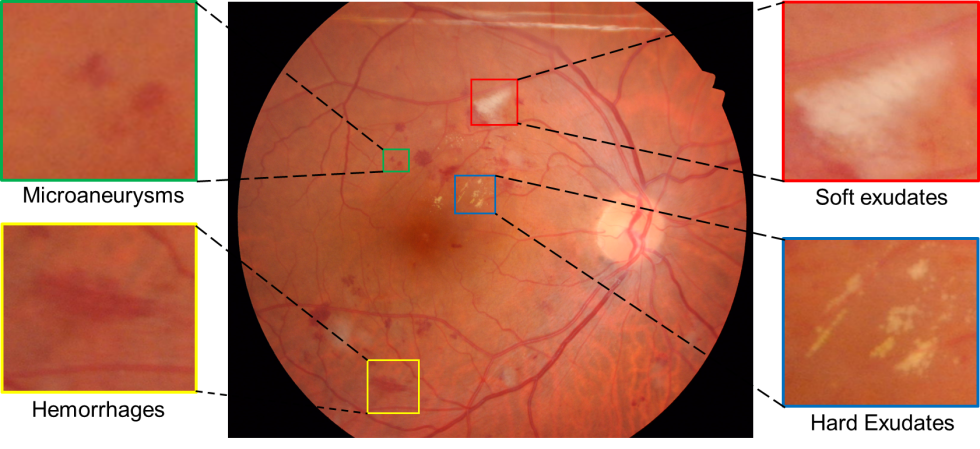
\includegraphics[width=1.0\textwidth]{figure/biomarker_localization_example}
	\caption[眼底图像中视网膜糖尿病病变对应的多种疾病标记物示例]{眼底图像中视网膜糖尿病病变对应的多种疾病标记物示例。} 
	\label{fig:biomarker_localization_example}
\end{figure}
%\subsection{主要难点}\label{sec:difficulties}
%实现在弱监督条件下,对分布不规则,并且具有不同形状和大小的疾病标记物实现精确定位,临床意义重大,但是存在诸多难点。概括起来主要有以下三个方面:

%1)在实验数据方面,医学数据收集就比自然图像要困难。另外,由于要对实验结果进行定量分析,就必须提供金标准。不幸的是,糖尿病视网膜病变数据集作为开源数据集,本身只有图像级标签,并没有像素级标签,因此需要专业医师对数据进行标注。而糖尿病视网膜病变图像上的疾病标记物分布十分广泛、形状大小各异,再加上细小疾病标记物与背景之间的边界模糊,极易与背景混淆,因此,数据标注代价高昂。另外,视网膜图像上纹理丰富复杂,这也使得弱监督下条件的疾病标记物定位问题变得更加困难。

%2)在网络训练方面,由于本文网络结构中涉及到三个部分。其中还涉及到对抗生成网络的训练,而我们是想通过图像生成的方式来实现疾病标记物的精确定位。因此,对抗生成网络训练起着至关重要的作用。实际上,自2014年对抗生成网络提出以来,其训练过程就存在训练不稳定、梯度消失、模式崩溃等问题,而且损失函数无法指示训练过程和效果。虽然已有一些列改进方案~\cite{mirza2014conditional, radford2015unsupervised, arjovsky2017wasserstein, gulrajani2017improved, mao2017least},但是上述问题始终没有得到彻底解决。另外,如何将对抗生成网络和CNN分类器组合训练也是一个值得考虑的问题。在这方面,我们是没有直接经验可以借鉴的。

%3)在从二类问题推广到多类问题时,首先由于各类样本数量不一定相等或相近。因此,在训练过程中可能会出现类别不平衡问题。另外,由于在训练对抗生成网络时每次迭代判别器只能两个输入端(正例和负例),而异常类却有多个(数量$\geq 2$)。因此,如何组织数据训练对抗生成网络也需要考虑。一种方案是同时增加判别器至多个,但这会大大增加网络训练过程的复杂性和难度,同时会增加GPU等硬件资源的开销。另一种方案是不增加判别器数量,将所有异常类看做一个整体,保证迭代训练对抗生成网络时正例和负例整体数量相等。这样看似能完美解决,但实际上,在正例数量与负例中每一种异常类之间依然存在类别不均衡现象。

%鉴于上述三个方面的问题,在弱监督条件下,对分布不规则,并且具有不同形状和大小的疾病标记物的精确定位任务仍然比较棘手。
\section{论文结构与章节安排}\label{sec:arrangement}
本文将会用六章的内容,仔细而全面的介绍本文提出的精确定位疾病标记物方法,并在相关数据集上完成实验验证,各章内容安排如下:
%https://stackoverflow.com/questions/2740437/changing-style-of-latex-description-lists
%https://latex.org/forum/viewtopic.php?t=7607
\begin{description}[style=multiline,leftmargin=1.7cm]
	\item[第一章:] 绪论。本章将叙述与疾病标记物定位任务相关的背景知识。此外,我们还将概述本文的研究内容及其主要难点。
	\item[第二章:] 相关研究基础。本章将介绍后文用到的相关技术和相关研究进展。随后此章还将介绍后文实验中所使用的评价标准和与疾病标记物定位相关的主流数据集。
	\item[第三章:] 疾病标记物的自动定位方法。本章将详细描述我们针对疾病标记物定位任务提出的解决方法。具体而言,本章将首先描述本文的研究问题和解决思路,据此我们给出本文提出的方法、模型结构、训练策略和损失函数。最后,本文将用一张算法流程图用形式化语言描述网络训练过程。
	\item[第四章:] 二类疾病标记物定位的实验评估。本章将利用本文提出的模型在两个二类数据集上进行相关实验。本文还将针对本文提出的模型本身,设计一系列消融实验。最后,本文设置多组不同的实验参数,以探讨本文提出的方法的鲁棒性。
	\item[第五章:] 多类疾病标记物定位的实验评估。与第四章类似,此章将利用本文提出的模型在一个多类数据集上进行相关实验。
	\item[第六章:] 总结与展望。此章将对全文工作进行总结性描述,并明确未来研究方向。
\end{description}